\chapter{Evaluation}

With an implementation of Multi--Paxos having been developed it is now necessary discuss its evaluation; both in terms of its ability to perform under the assumptions of the environment in which it operates and also to characterise its performance in a number of typical cases.

\section{Experimental setup}

This section describes the framework upon which simulations were setup to allow for evaluation to take place.

\subsection{Experimental measurements}

Performance evaluation requires the measurement and subsequent analysis of experimental data. There are two key metrics required for evaluating the performance of networked systems -- \emph{latency} and \emph{throughput}. \\

\textbf{Latency} is the time taken elapsed  between a client sending a request to the system and receiving a response. It is measured by a client broadcasting a command with a \texttt{Nop} operation to the set of replicas and starting a timer. The timer is stopped when the response with the corresponding command identifier is received and the elapsed time is calculated and output to a trace log file. \\

\textbf{Throughput} is the rate at which the system services requests and hence measured in requests per unit of time. Clients submit requests at a fixed rate (e.g. 10 requests per second) and the number of responses returned per second is measured by clients. This gives a throughput for a given arrival rate and allows for a peak throughput measurement to be made. That is, a certain arrival rate of requests will maximise the output throughput which represents the maximal rate at which the system services requests. \\

\subsection{Mininet}

Mininet is the network simulator that was used for the evaluation of the implementation. Mininet comes with a Python API that allows for scripts to run network simulations. Mininet allows for arbitrary Linux processes to be run on any of the virtual hosts. This involved installing an OCaml runtime to execute bytecode compiled on the development machine. The simulation runs Python scripts that performs simulations that proceeds as follows

\begin{enumerate}
  \item Setup up network topology, populating it with hosts and switches and their interconnects (and the performance parameters)
  \item For a given number of each role participating, a JSON configuration file is generated that lists each host IP address and port number
  \item Multi--Paxos instances are started via the OCaml runtime on each virtual host with their parameters set (e.g. whether they are clients)
  \item The simulation starts and proceeds to execute for a given amount of time
  \item The simulation is terminated. Configuration files are deleted and the virtual network is torn down and each process is terminated.
\end{enumerate}

Log files are saved by each process on a shared filesystem with the host machine upon which they are analysed by another Python script which produces plots using matplotlib\footnote{https://matplotlib.org/}.

{\color{blue}Perhaps a diagram here showing the workflow of how we use Mininet.}

\subsection{Duelling leaders and the impossibility result}

\begin{figure}
  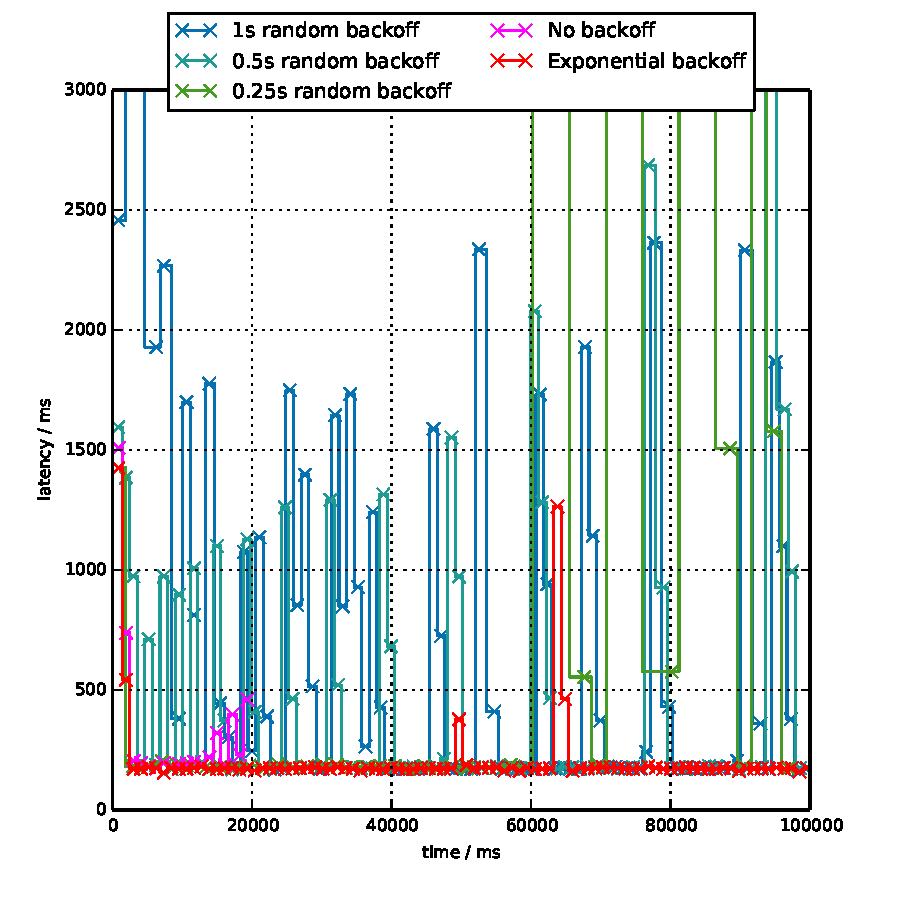
\includegraphics{include/backoffs.pdf}
  \caption{Graph of backoffs}
  \label{fig:backoff-graph}
\end{figure}

When performing initial experiments on the system it became apparent that systems that have more than one leader would regularly livelock when processing requests from clients. Inspection of log files led to me finding out this was a well--known case of \emph{duelling leaders}. This occurs when leaders will attempt to gain adoption of their ballot but are preempted by another leader. The leader will then attempt to gain adoption of another ballot before the other leader's ballot is accepted, causing the other leader to attempt adoption of a higher ballot. The leaders will continually increment their ballots and seek adoption without any given ballot being accept, livelocking the system and leaving it unable to make progress. \\

There is a well known result called the FLP Impossibility result, outlined in Fischer et al's paper \cite{Fischer:1985:IDC:3149.214121} that proves that consensus is never guaranteed in an asynchronous environment that permits crash failures. The problem of duelling leaders is an instance of this problem and so there is no guarantee that consensus can be reached in an asychronous environment. \\

However, there are methods to vastly reduce the chance that leaders will duel. One simple method is to have a \emph{random backoff} so that each leader will pause their operation for a random amount of time in some range. This increases the chance that a leader will have its ballot accepted before being preempted by another leader. A slightly more sophisticated method is to employ \emph{exponential backoff}. In this case each leader will employ a random backoff within some range and upon being preempted this range is doubled. The backoff time is reduced to an initial value when an adopted message is received by a leader. This reduces the amount of idle waiting that may occur when using a random backoff and no duelling is occurring. \\

Figure \ref{fig:backoff-graph} shows a number of traces with different backoff strategies. With no backoff, the system halts at after 18 requests are processed and makes no further progress processing requests as the leaders duel. Three traces of random backoffs with different maximum wait times were collected. With greater maximum wait times there are a number of greater sporadic delays in the system as these leaders often have to wait idly even when duelling is not occuring. Making the random timeout too small, as in the 0.25s case, reduces the number of delays but increases the chance leaders will duel for some time before one waits long enough for the other to make progress, resulting in very large delays. The exponential backoff (starting with a value of 0.25s) performs best, with very little delay in the general case and ocassional delays as backoff windows increase in size when a duelling situation occurs.

{\color{green}\section{Simulation tests}

Define here what we  meanby simulation tests: tests that ensure the expected behaviour of the system as a whole is undertaken. \\

Explain this fits into our definitions of what a test harness is and how we're going to use that to perform evaluations. Explain this also requires modification of the program to ensure we can crash / delay acceptors suitably so as to simulate the sort of failure modes we require. \\

Perhaps describe a system test and then also reference a table describing each test in the appendix. \\}

\subsection{Topologies}

\begin{figure}
  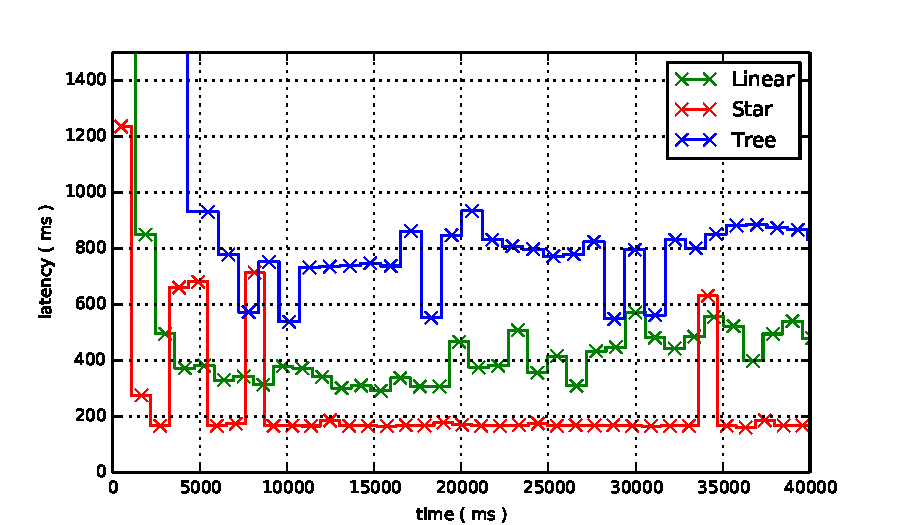
\includegraphics{include/topos.pdf}
  \caption{Graph of topologies}
  \label{fig:topo-graph}
\end{figure}

An important consideration when evaluating the system on a simulated network is to ensure that the results collected do not reflect the characteristics of the network itself rather than reflecting the characteristics of the system itself. For example we do not wish for delays in queues at switches to dominate the measurements of latency for the system itself. An initial experiment was performed to observe the steady state behaviour of the system with three different network topologies, shown in {\color{red}show diagram}. Topology (a) represents a star topology wherein each host is connected to a single switch. Topology (b) represents a linear network wherein each process with the same role is connected to a single switch and these are each connected together. Topology (c) represents a tree topology with switches arranged in a binary tree structure. \\

Figure \ref{fig:topo-graph} shows the traces produced when measuring the steady state latency of each topology. No unexpected behaviour occurs in any of the three schemes. The main difference to note is that the average latency of each trace varies between each topology. This is because the number of hops from each sender and receiver participating in the system varies. For example, every host is two hops away in the star topology, 3 hops away in the linear topology and a variable number of hops away in the tree topology. There is no unexpected queuing behaviour resulting in very large delays for any of the given topologies. \\

\section{Performance evaluation}

Introduction to the performance evaluation.

\subsection{System size}

Describe the network architecture; describe the no of clients, the messages they send, how many they send; rate of sending. Explain we want to avoid measuring delays in links and delays in dropped packets in queues etc. \\

Describe how we want to measure commit latency and throughput as the number of different nodes in the system is varied. Achieve this by varying number of nodes and measuring latency and throughput. \\

Explain the confidence interval calculations. \\

{\color{blue}Should end up with two bar charts for latency and throughput as a function of cluster size. Plot LibPaxos values for each as well} \\

Compare performance to LibPaxos.

\subsection{Failure traces}

Describe how we need to assess the system in the case of failures. \\

Talk about computation of means, EWMA, etc. \\

$$ \textrm{EWMA} \left( t \right) = \alpha \times \textrm{RTT} + (1 - \alpha ) \times \textrm{EWMA} \left( t - 1 \right)$$

{\color{blue}Replica failure traces. Include plain failures, failures including restarts and cascading failure until we get no further latency and throughput. Include LibPaxos traces over the time. Should result in six graphs if we're lucky.} \\

Compare performance to LibPaxos.


%\section{Experimental Setup}
%\subsection{Mininet}
%\begin{itemize}
%  \item Describe the simulation framework used with Mininet - how the simulation scripts are structured.
%  \item Describe the system by which a simulation is performed - include a diagram of how simulation scripts and executable binaries are transferred to the simulation, simulations are performed %and resulting log files are returned to the host-machine for analysis and plotting.
%  \item Describe the system by which tracing is performed.
%\end{itemize}

%\subsection{Libpaxos}
%\begin{itemize}
%  \item Short description of Libpaxos library.
%  \item Explain how application was written / any modifications necessary to run the same sample application.
%\end{itemize}

%\section{Steady state behaviour}
%\begin{itemize}
%   \item Characterise the steady state behaviour of the system - capturing the latency and throughput in a given configuration. Plot against each other to show characteristics.
%   \item Comparison in the steady state behaviour between the project implementation and Libpaxos.
% \end{itemize}

% \section{Configuration sizes}
%\begin{itemize}
   %\item Treatment of experiments that describe how latency and throughput vary as a function of the number of different nodes in the configuration varies.
    %\item Include description of the exact experiment performed and how confidence intervals were calculated.
   %\item Include graphs for: latency against different cluster sizes and throughput against different cluster sizes. Include Libpaxos version of this as well.
%\end{itemize}

%\section{Failure traces}
%\begin{itemize}
%  \item Experiment pertaining to crashing a replica and observing system behaviour over time.
%  \item Describe how data was averaged - including the sample mean and EWMA.
%  \item Graph of latency and throughput as a function of time with a specific point a replica is crashed noted.
%  \item Similar graph with a replica restoration.
%  \item Graphs / on the same plot with behaviour of Libpaxos.
%\end{itemize}

%\section{Quorum sizes}
%\begin{itemize}
%  \item ...
%  \item ...
%\end{itemize}

\section{Summary}
